\documentclass[../../../main.tex]{subfiles}
 
\begin{document}

\begin{table}
\centering
\begin{tabular}{| c | c | c | c | c |}
\hline \hline
Semester & Course & Credits & Students & Curriculum feature \\ \hline
Fall 2017 & PHYS135A-01 & 4.0 & 24 & Intro \\ \hline
Fall 2017 & PHYS150-01 & 4.0 & 17 & COM1/Intro \\ \hline
Spring 2018 & PHYS135B-01 & 4.0 & 18 & Intro \\ \hline
Spring 2018 & PHYS180-02 & 5.0 & 19 & COM1/Intro \\ \hline
Spring 2018 & COSC330/PHYS306 & 3.0 & 6 & Advanced \\ \hline
Fall 2018 & PHYS135A-01 & 4.0 & 24 & Intro \\ \hline
Fall 2018 & PHYS135A-02 & 4.0 & 26 & Intro \\ \hline
Jan 2019 & COSC390 & 3.0 & 8 & Advanced \\ \hline
Spring 2019 & PHYS135B-01 & 4.0 & 25 & Intro \\ \hline
Spring 2019 & PHYS180-02 & 4.0 & 9 & Intro/COM1 \\ \hline
-- & Total & 39.0 & -- & -- \\ \hline
\hline
\end{tabular}
\caption{\label{tab:courses:teaching} This table is a summary of the courses I have taught since Fall 2017.  The introductory courses carry the course numbers 135A, 135B, 150, and 180.  The advanced course PHYS306 is cross-listed as a computer science course, COSC330. The other advanced course, COSC390, is now listed as an upper division computer science course and counts towards the Integrated Computer Science (ICS) requirements.  This table does not include the two times I have taught PHYS396 (Physics Research), which does not count for teaching credit, but is 3.0 credits per student.  Physics 396 also goes toward \textbf{Departmental goal 2}.}
\end{table}

\textbf{\textit{Algebra-based physics (135A/B)}}. Algebra-based physics, PHYS135 A/B, is a two-semester integrated lecture/laboratory sequence that covers algebra-based physics from kinematics and Newton's Laws to electromagnetism without the mathematics of calculus\footnote{See supplemental material for example syllabi.}.  Algebra-based physics is a core requirement for many technical majors such as kinesiology (KNS) and chemistry (CHEM).  Students learn problem solving in a physics context with algebra, trigonometry, and vectors.  I employ a mixture of traditional and PER active learning methods to \textbf{satisfy departmental goals 1, 4, and 6}.  These methods are \textit{Peer Instruction (PI)} and \textit{Physics Education Technology (PhET)}.  I no longer use JITT modules, which I experienced to be ineffective for the students (see Sec. \ref{sec:oof}).  I attended the American Association of Physics Teachers (AAPT) Workshop in 2017 to practice the implementation of these modules \footnote{See supplemental material for details.}, and I have since modified them as per department and FPC recommendations.  My total teaching credits and number of students for this course is listed in Tab. \ref{tab:courses:teaching}.  \\ \hspace{0.1cm}

The first learning focus I identify for non-majors is \textbf{curiosity}, with the measureable goals stated in Sec. \ref{sec:teaching_phil1}.  To help satisfy the goal of increasing their interest in physics, I encourage an activity at the beginning of each class period in which a student presents a news or science journal article pertaining to physics that was published in the previous week.  I incentivise the students to volunteer as presenters by offering extra credit, and through the activity I help them to practice oral communication of scientific ideas (\textbf{Departmental goal 7}) and help them recover points lost on midterms \footnote{Examples of such articles presented by students are included in the supplemental materials.}. \\ \hspace{0.1cm}

A second method I use to increase student curiosity is to require the students to design and complete a physics experiment.  The OpenStax textbooks contain many workable suggestions that the students can construct.  Each student group must first collectively agree on an idea, and submit a proposal to me in the middle of the semester.  I then edit it with the group and ensure they have the equipment they need.  After they have begun to collect data, I invite them to office hours to coach them on the presentation of the results \footnote{Included in the supplemental materials are examples of the students' final presentations.}.  By allowing the students to choose the topic and design, I provide them the opportunity to satisfy their own curiosity.  Making this assignment an oral presentation also goes toward \textbf{Departmental goal 7}.  With the two activities of article/journal presentations, and group-designed physics labs, I touch upon all three goals for the curiosity learning focus.  The data in Sec. \ref{sec:oof} show that the students are reporting an increase in their curiosity for physics at an increasing rate over time. \\ \hspace{0.1cm}

The second introductory course learning focus is \textbf{improvement of analysis skill}.  PI (Peer Instruction) modules were first developed by Eric Mazur \cite{mazur2013peer}, and tend to yield higher learning gains than traditional lecture content.  Moreover, it is often helpful to illustrate physics concepts with PheT (Physics Education Technology) simulations, or to perform laboratory activities we cannot consruct (e.g. altering the strength of gravity) \cite{phet}.  These two activities form the engine by which I seek to improve the analysis skill of introductory students.  In alignment physics department and FPC recommendations, I have balanced the use of these two modules with the inclusion of more traditional lecture content in recent semesters.  Finally, after reflecting upon the use of JITT modules \cite{jitt}, I have decided to cut them in favor of more example problems.  The students express a desire for more concrete, step-by-step examples.  Although popular PER methods claim to yield better results than traditional content, we must be receptive to the concerns of the students. \\ \hspace{0.1cm}

A typical introductory physics class in the lecture/laboratory format begins with 1-2 journal/news article presentations from the students.  After a short discussion, we begin with a warm-up example on the white board from the prior class.  We then introduce new concepts on the projector screen, followed by several examples worked out in traditional form by me on the whiteboard.  Third, I engage the students with a PI module pertaining to the topic at hand.  PI modules first pose a problem \textit{conceptually}, with A-D multiple choice answers.  Our classrooms are equipped with a system that records student answers anonymously.  The students take several minutes to think conceptually \textit{without specific numbers or equations}, and answer on their own.  I view the answer distribution, and if fewer than 70\% of the class answers correctly, I ask them to discuss at their table how they obtained the answer.  The students often learn best from each other, as they explain their reasoning in their own words.  I circulate through the classroom at this stage, seeking out the struggling students and helping them.  Deliberately focusing on the struggling students helps me to build a relationship of trust with them, and relaxes anxieties they have with word problems.  \\ \hspace{0.1cm}

After 2-3 minutes, I require them to re-submit their answers \textit{as a group} at their table.  We observe the distribution of answers (choices A-E) \textit{shift} toward the correct one at the end of PI modules\footnote{See supplemental material for example PI modules.}.  Further, if the students answer correctly before the group discussion I learn that I can move on without the need for the group discussion.  In this way, we only accelerate the pace when most of the students are ready.  This leads to the possibility of 1-2 students being left behind (if they are not in the super-majority of the A-D answers), so I have added the concept of WAT\footnote{e.g. ``What?'' A meme indicating confusion.}.  Usually WAT corresponds to answer E, and it allows a student who is lost notify me anonymously.  If a WAT occurs, I work another example until it disappears.  \textit{This strategy ensures inclusivity in my introductory classes}, in that we leave no struggling student behind.  For more difficult or extended examples, I have the student groups work the problem together on the whiteboards in the classroom together\footnote{I named this trick ``board problems'' in my previous PEGP.}. The advantage there is that the students can observe how other groups are solving a problem step-by-step. \\ \hspace{0.1cm}

The second-half of the lecture/laboratory format moves on to the laboratory activity or PheT module.  An example of the difference between traditional labs and PhET modules occurs in PHYS135B and PHYS180, which cover electromagnetism.  In these courses, we often build DC electric circuits.  If the circuit is constructable in our lab, we perform a traditional experiment in which we measure voltages and electric current to verify a principle such as Ohm's Law.  If the circuit cannot be easily built in our lab, we simulate it virtually with PhET software.  Whenever possible, we first simulate the circuit in PhET, and then construct it to compare theory and experiment in full detail.  The PI modules, PheT modules, and traditional lecture content complete my strategy for improving the students' analysis skill, and go towards \textbf{Departmental goals 1, 4, and 6}.  \textit{The student evaluation data in Sec. \ref{sec:oof} show great progress in a broad range of measures in this category.} \\ \hspace{0.1cm}

I employ several methods to reach my third introductory course learning focus, \textbf{applications to society}.  The obvious routes are the applications in the OpenStax texts \cite{openstax1} regarding kinesiology and medicine.  I develop special PI modules and example problems around topics such as motion/work/energy in the human body, nerve cells as DC circuit simulation, and lightning/weather.  Which modules I deploy depends on the semester.  I have reflected on the fact that in more recent semesters I have been much better about learning what interests the students and including content specifically for the students in my class.  Another reason why I have dropped the JITT module is that it frees up time before class for me to add material I know particular students will enjoy\footnote{See supplemental material for an example of such a unit.}. \\ \hspace{0.1cm}

Two final methods for my third learning focus are the student-led article discussions, and term-papers.  A nice example of the former occured during the past year occurred when I had an environmental science major interested in climate change in PHYS135A/B who would find climate science articles that used concepts from class to present to the group.  This type of activity empowers the students to choose topics they value, and believe have an impact on our community.  Occasionally I give hints at articles which are of high-impact for the \textit{scientific community}, and this prompt is all most timid students need to take the next step of preparing one for class.  For extra-credit I offer term-papers asking students to explain the physics of a recent or past historical discovery.  Some brilliant examples have emerged, including the history of the first measurements of the distance between the Earth and the Sun\footnote{Included in the supplemental material.}.  The preparation of these papers requires the students to use concepts learned during the semester to understand scientific breakthroughs, as well as providing them a venue to practice writing about societal impact of physics (\textbf{Departmental goal 7}).  \\ \hspace{0.1cm}

\textbf{\textit{Calculus-based physics (150/180)}}. Calculus-based physics, PHYS150/PHYS180, is a two-semester lecture/laboratory formatted sequence that covers calculus-based kinematics, mechanics, work/energy, and electromagnetism\footnote{See supplemental material for example syllabi.}.  I employ a mixture of traditional and PER active learning methods to \textbf{satisfy departmental goals 1, 4, and 6}.  As in the algebra-based classes, I implement \textit{Peer Instruction (PI)} \cite{mazur2013peer} and \textit{Physics Education Technology (PhET)} \cite{phet} modules when necessary.  Because PHYS150 and PHYS180 require tools from single and multi-variable (vector) calculus, students taking those courses concurrently benefit from PhET simulations to help visualize calculus concepts.  Examples include operations with scalar and vector fields in electromagnetism, single-variable integrals and derivatives in kinematics, and line integral calculation of work and energy. My total teaching credits and number of students for this course is listed in Tab. \ref{tab:courses:teaching}. \\ \hspace{0.1cm}

My PHYS150/180 classes are taught with the same methods and format as the algebra-based courses, with the inclusion of the full calculus-based version of introductory physics concepts.  Since the subjects of calculus and Newton's Laws were developed concurrently, often by the same scientists, these two subjects are linked.  During the warm-up phase of class, I will sometimes pose a calculus problem (when necessary) to familiarize the students with a technique that is required to understand the concepts we will encounter during class.  Occasionally (and this is especially true in PHYS180) the physics requires calculus concepts that the students have not encountered yet in their concurrent courses.  These cases usually involve vector calculus (Calculus III, or MATH241), which helps to explain electric and magnetic fields.  I gauge the comfort level of the students, and typically restrict my vector calculus content via traditional whiteboard content and examples.  \textit{As a rule, we do not place calculus concepts on exams that the students have not encountered in pre-requisite or concurrent courses}.  \\ \hspace{0.1cm}

In Sec. \ref{sec:oof}, I reflect on the student evaluation data in the same fashion as with the algebra-based courses.  Similar to the conclusions for PHYS135A/B, the data in Sec. \ref{sec:oof} show that calculus-based student date shows an increase in their curiosity for physics over time, and \textit{great progress in measures touching upon their problem solving skills.}  I received almost perfect scores for data collected from my most recent PHYS180 course.  Although the reduced class size made this easier to achieve, I have reflected on the fact that the students place a high value on \textit{building a relationship of trust with them} in order to satisfy their curiosity and increase their analysis abilities. \textbf{Include examples of final projects.} %Review their written responses.

%To reach the first learning focus I identify for non-majors, \textbf{basic curiosity}, I use the three research-based methods plus a few other techniques.  For example, PhET simulations allow us to visualize the electric field generated by a specific charge distribution.  I can combine the field visualization with a PI module that asks the students conceptual questions about the field, including what geometric symmetry is being displayed and why.  Symmetry is an important topic in physics, but some students might not see it from equations or diagrams.  Group projects in calculus-based physics have generally been more sophisticated.  For example, students used the 3D printer to build a Sterling engine as a study of thermodynamics.  Another group studied 2D kinematics with air-pressure rockets on the football field.  A side benefit of these presentations is that the students practice good \textit{oral communication.} \\ \hspace{0.1cm}

%To reach the second of the three learning focuses, \textbf{improvement of analysis skill}, I utilize the peer instruction method (PI modules), in conjunction with a procedure I learned on the fly during my first semester.  I require the students to \textbf{leave their tables, and solve the technical or numerical problem together on the whiteboards} that cover the walls of my classrooms.  Students are able to see each other's approach, and validate it against their own group's method.  Upon returning to the tables, the groups feel more prepared and eager to solve the PI module problems that follow.  The students report in their evaluations that adding this step greatly benefited their learning, and that they felt more comfortable with the material afterwards.  The students also gain analysis experience via the process of understanding statistical and systematic measurement errors.  Relative to the algebra-based activities, the calculus-based activities require a more complete understanding of error propagation. \\ \hspace{0.1cm}

%To reach my focus of \textbf{applications to society}, I begin with the prompts to applications in the OpenStax texts, creating units that are relevant for the majors in my class.  Examples have included nerve signals, solar wind, and global warming.  The JITT modules demonstrate if the students have done the reading I assign, and whether they comprehend how the physics we are learning applies to society. The term-papers asking students to explain the history of science for a given topic also serve this teaching focus.  The Nobel Prize in Physics last year was for the discovery of gravitational waves, and several students chose to write about Advanced LIGO, the experiment that recorded the famous signals that have now broadened society's understanding of general relativity.  Group presentations on self-designed science projects at the end of the course offer a chance to practice oral communication skills.  Finally, I required in PHYS180 each student to briefly summarize a scientific journal article for the class, in an attempt to further practice oral communication of science. \\ \hspace{0.1cm}

\subsubsection{Descriptions of each Module Type}

The following descriptions provide more detail about our PER instructional modules, in list form.

\underline{PI Modules} - Implementation of an active learning strategy involving group problem solving and discussion.  Several good references are found in \cite{mazur2013peer} \cite{AAPTPI} \cite{PhysPort}.
\begin{itemize}
\item PI-based modules contain conceptual, multiple-choice questions for the class about a physical system.  The question corresponding to the results in Fig. \ref{fig:exampleData} was \\ \vspace{0.5cm} \textbf{``If the slope on a position vs. time graph is positive before a time $t_0$, zero at $t_0$, and negative after $t_0$, which of the following is true? \\ \vspace{0.5cm} A) The acceleration of the object was negative before and after $t_0$.  \\ B) The acceleration of the object was positive before $t_0$, then negative. \\ C) The acceleration of the object was positive before and after $t_0$. \\ D) The object had no acceleration.}
\item Students respond \textit{individually and anonymously} with an electronic device, and the distribution of answers for choices A-D is shown on the class screen (see Fig. \ref{fig:exampleData}).
\begin{figure}
\centering
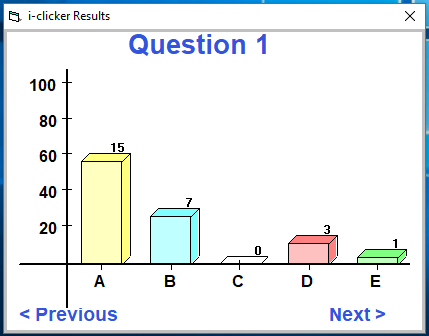
\includegraphics[width=0.45\textwidth,trim=0.25cm 1cm 0.15cm 2cm,clip=true]{FirstData.PNG}
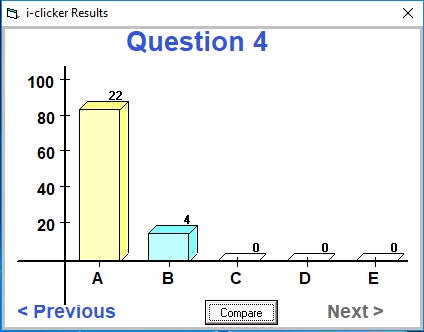
\includegraphics[width=0.45\textwidth,trim=0.25cm 1cm 0.15cm 2cm,clip=true]{SecondData.PNG}
\caption{\label{fig:exampleData} (Left) An answer distribution of my 25-student introductory algebra-based physics class, for a question that had a correct answer of A.  This distribution triggered a table discussion, because the fraction of correct answers was 0.6.  In addition, one student pressed E, indicating they were confused.  This prompts the professor to give a clue, or work another example.  (Right) After a table discussion with their peers, the students responded a second time, and the fraction of correct answers rose to 22/25 = 0.88.  The key concept for the question is that velocity and acceleration are not the same quantity (see text).}
\end{figure}
\item Students know to answer E if they are confused, and the anonymity is ensured so that students feel comfortable and the class is made more inclusive.
\item One of two actions is taken next:
\begin{enumerate}
\item If the fraction of correct answers to the conceptual question is larger than 0.7, class proceeds to the next exercise or new material.  This was the recommended fraction at the AAPT conference I attended in 2017.
\item If the fraction is less than 0.7, the professor initiates \textbf{table discussion}.
\end{enumerate}
\item \textbf{Table discussions} take place between students at the same table.  During this time the professor circulates, searching for the struggling students and answering questions.  After approximately 3-5 minutes, the discussion ends.
\item A second poll of the class is taken after table discussions, if they take place.  The \textit{shift} in the distribution towards the correct answer indicates an improved understanding of the concepts.  If the shift is not observed, the professor takes appropriate action.  If more than one person selects E, the material is covered again regardless of the shift.
\item The overall procedure is repeated for several exercises, and table discussions take place when necessary.  After several exercises, the class proceeds to new material, or the next concept in the unit.
\end{itemize}

\underline{PhET Modules} - Simulations written in HTML and JAVA, and published by The University of Colorado, Boulder, with public support from the National Science Foundation and private support from Google and the Moore and Hewlett Foundations \cite{phet}.  The goals of the simulations are that anyone should be able to operate them, and that they be based on proven PER.  The benefits of the simulations are researched and they are only published if the benefits to the students has been proven.
\begin{itemize}
\item The OpenStax textbooks for PHYS135 A/B and PHYS150/PHYS180 have built-in links to PhET simulations that allow students to illustrate concepts by visually simulating physics systems.
\item Several HTML5-based examples are here:
\begin{enumerate}
\item Electric charge and electric field: \url{https://phet.colorado.edu/en/simulation/charges-and-fields}
\item DC circuit construction: \url{https://phet.colorado.edu/en/simulation/circuit-construction-kit-dc}
\end{enumerate}
\item PhET simulations are incorporated into active learning in the classroom in four situations:
\begin{enumerate}
\item When a PhET simulation re-creates a laboratory measurement we are about to perform, it is useful to first simulate the expected results with the HTML or Java code and then perform the measurement to confirm the behavior of the system.
\item PhET simulations are also used when a desired measurement or experiment cannot be performed or constructed in the lab, such as altering gravity or changing the amount of friction between two surfaces.  Students benefit by being able to ``fine-tune'' a system, in order to expose the behavior of a system in real time.
\item PhET simulations are used to \textit{visualize} physical objects which are invisible.  Obvious examples are magnetic, electric, and gravitational fields, which are real but not (always) visible.
\item In special units, such as studying the behavior of electrical signals in the human body, there are PhET simulations from other fields (biology, chemistry, earth science, etc.) that prove useful to engage students' curiosity.
\end{enumerate}
\end{itemize}

\end{document}

